% See exam.cls and examdoc.tex for the license information
\documentclass[12pt, answers]{exam}

\usepackage{amssymb}
\usepackage{makeidx}
\usepackage{amsmath}
\usepackage{graphicx}
\usepackage{caption}
\usepackage{tabulary}
\usepackage{color}
\usepackage{multicol}
\usepackage{float}
%\usepackage{multirow}
%\usepackage{enumerate}

\usepackage{array}
\newcolumntype{C}[1]{>{\centering\let\newline\\\arraybackslash\hspace{0pt}}m{#1}}

\addpoints

% In case we're not using hyperref.sty:
\providecommand{\texorpdfstring}[2]{#1}
% The following can be used in \section commands
% without generating pdf warnings:
\newcommand{\bs}{\texorpdfstring{\char`\\}{}}

\makeindex

\newcommand{\indc}[1]{\index{#1@\texttt{\char`\\#1}}}
\newcommand{\indcsub}[2]{\index{#1@\texttt{\char`\\#1}!#2}}
\newcommand{\indcstart}[1]{\index{#1@\texttt{\char`\\#1}|(}}
\newcommand{\indcstop}[1]{\index{#1@\texttt{\char`\\#1}|)}}

\newcommand{\indt}[1]{\index{#1@\texttt{#1}}}
\newcommand{\indtsub}[2]{\index{#1@\texttt{#1}!#2}}
\newcommand{\indtstart}[1]{\index{#1@\texttt{#1}|(}}
\newcommand{\indtstop}[1]{\index{#1@\texttt{#1}|)}}

\extraheadheight{-.4in}

\pagestyle{headandfoot}
%\extraheadheight{.2 in}
\firstpageheader{}{}{}
\runningheader{}{}{}
\firstpagefooter{}{Extension of global alignment}{Page \thepage\ of \numpages}
\firstpagefootrule
\runningfooter{}{Extension of global alignment}{Page \thepage\ of \numpages}
\runningfootrule

%---------------------------------------------------------------------

\shadedsolutions
\noprintanswers
\definecolor{SolutionColor}{rgb}{0.8,0.9,1}

\setcounter{section}{2}

\begin{document}

\section{Exercises -- Extension of global alignment}

%---------------------------------------------------------------------
\begin{questions}

%%% Question 1
\question \textbf{DP with score matrix}
  
Use the score matrix below with gap penalty g =1 and answer the following questions.

\vspace{0.1 in}

\begin{figure}[h]
  \centering
      \includegraphics[width=0.2 \textwidth]{fig03/simple_score_matrix.png}
\end{figure}

\begin{parts}

%% (a)
  \part	Calculate the alignment score.

\begin{itemize}
\item Alignment 1
\begin{verbatim}
    q: ATGCT
    d: CA--T \end{verbatim}
    
\begin{solution}[0.35 in]
  1
\end{solution}
  
\item Alignment 2
\begin{verbatim}
    q: CAGCT
    d: C-A-T \end{verbatim}
  
\begin{solution}[0.35 in]
  1
\end{solution}

\end{itemize}

%% (b)
\part Calculate the score of $H_{i,j}$.

\begin{itemize}
\item Table A
\begin{figure}[h]
  \centering
      \includegraphics[width=0.25 \textwidth]{fig03/cell_update_score_matrix_1.png}
\end{figure}

\begin{solution}[0.35 in]
1
\end{solution}

\item Table B
\begin{figure}[!h]
  \centering
      \includegraphics[width=0.25 \textwidth]{fig03/cell_update_score_matrix_2.png}
\end{figure}

\begin{solution}[0.35 in]
1
\end{solution}

\end{itemize}

\pagebreak

%% (c)
\part Fill the empty cells with appropriate scores in the DP table. What is the optimal alignment score?

\begin{figure}[h]
  \centering
      \includegraphics[width=0.35 \textwidth]{fig03/dp_with_score_matrix.png}
\end{figure}

\begin{solution}[0.75 in]
1
\end{solution}

%% (d)
\part There are two different alignments that give the same optimal score in the solution above. Specify both of them.

\begin{solution}[1.75 in]
\begin{verbatim}
  q: CAGCT
  d: CA--T
  
  q: CAGCT
  d: C-A-T
\end{verbatim}
\end{solution}

\end{parts}


\pagebreak

%%% Question 2
\question \textbf{Affine gap penalty}
  
Affine gap penalties are often preferable ways to calculate gap scores than linear penalties. A gap with length l can be calculated as: $g_{l} = g_{open} + (l - 1) * g_{extend}$.

Use the following scoring scheme and gap penalties to answer the questions.

\textbf{Scoring scheme: }\\
\null \quad $R_{ab}$ = 1 for a = b \\ 
\null \quad $R_{ab}$ = 0 for a $\neq$ b \\ 
\null \quad $g_{open} = 1$, $g_{extend} = 0.1 $ 

\vspace{0.1 in}

\begin{parts}

%% (a)
  \part
  What is the gap penalty when $l = 2$.
    
  \begin{solution}[0.35 in]
  $g_{l=2} = 1+ (2 - 1) * 0.1 = 1.1$
  \end{solution}

%% (b)
  \part
  Calculate the scores of the alignments.
  
\begin{enumerate}
\item 
  \begin{verbatim}
    q: CAGCT
    d: CT--T \end{verbatim}
    
  \begin{solution}[0.35 in]
  0.9
  \end{solution}
  
\item 
  \begin{verbatim}
    q: CAGCT
    d: C-T-T \end{verbatim}

  \begin{solution}[0.35 in]
  0
  \end{solution}
      
\item 
  \begin{verbatim}
    q: CCT--
    d: ---CT \end{verbatim}

  \begin{solution}[0.35 in]
  -2.3
  \end{solution}
      
\end{enumerate}  
 
  \vspace{0.1 in}

\end{parts}

%%% Question 3
\question \textbf{Affine gap with single DP table}
  
You need to check extra cells in addition to the adjacent cells of H when finding an optimal alignment with affine gap penalties.

\medskip 

\textbf{Scoring scheme: }\\
\null \quad $R_{ab}$ = 1 for a = b \\ 
\null \quad $R_{ab}$ = 0 for a $\neq$ b \\ 
\null \quad $g_{open} = 1$, $g_{extend} = 0.1 $ 

\begin{figure}[h]
  \centering
      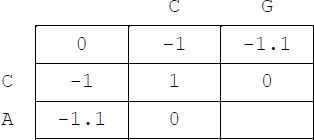
\includegraphics[width=0.3 \textwidth]{fig03/affine_gap_single_table.png}
\end{figure}

Assume we want to update $H_{2,2}$ and answer the following questions.

\newpage

\begin{parts}

%% (a)
  \part
  Calculate $H_{1,1} + R_{q_2, d_2}$.
    
  \begin{solution}[0.35 in]
  $1 + 0 = 1$
  \end{solution}

%% (b)
  \part
  Calculate $max_{1 \leq l \leq 2}(H_{2,2-l} - g_{l})$.

  \begin{solution}[0.35 in]
  $max⁡(H_{2,1} - g_{l=1}, H_{2,0} - g_{l=2}) = max(0 - 1, -1.1 - 1.1) = -1$
  \end{solution}
  
%% (c)
  \part
  Calculate $max_{1 \leq l \leq 2}(H_{2-l,2} - g_{l})$.

  \begin{solution}[0.35 in]
  $max⁡(H_{1,2} - g_{l=1}, H_{0,2} - g_{l=2}) = max(0 - 1, -1.1 - 1.1) = -1$
  \end{solution}
  
 %% (d)
  \part
  What is the score of $H_{2,2}$.
  
  \begin{solution}[0.35 in]
  $max(1, – 1,  -1) = 1$
  \end{solution}
     
  \vspace{0.1 in}

\end{parts}

%%% Question 4
\question \textbf{Initializtion for affine gap penalty}
  
Initialize the following tables when $g_{open} = 10$ and $g_{extend} = 1$.

\vspace{0.1 in}

\begin{figure}[h]
  \centering
      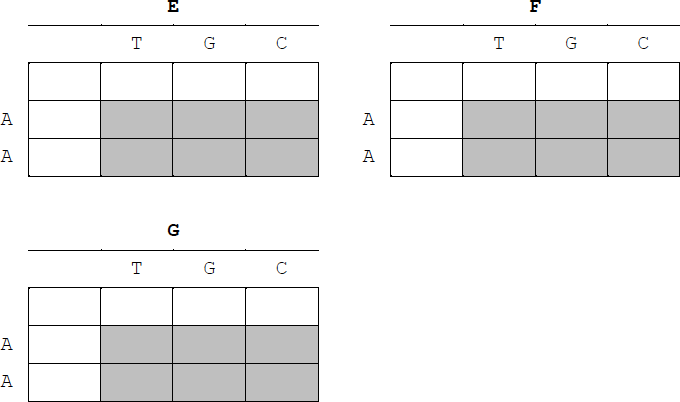
\includegraphics[width=0.7 \textwidth]{fig03/affine_dp_initialize.png}
\end{figure}

  \vspace{0.1 in}

%%% Question 5
\question \textbf{Affine gap with three DP tables}
  
Use the following scoring scheme and gap penalties to find the optimal alignment score of two sequences q = AG and d = GGGC.

\medskip 

\textbf{Scoring scheme: }\\
\null \quad $R_{ab}$ = 1 for a = b \\ 
\null \quad $R_{ab}$ = 0 for a $\neq$ b \\ 
\null \quad $g_{open} = 1$, $g_{extend} = 0.1 $ 

\vspace{0.1 in}
\newpage

\begin{parts}

%% (a)
  \part Fill all blank cells in the DP tables E, F, and G.
    
\begin{figure}[h]
  \centering
      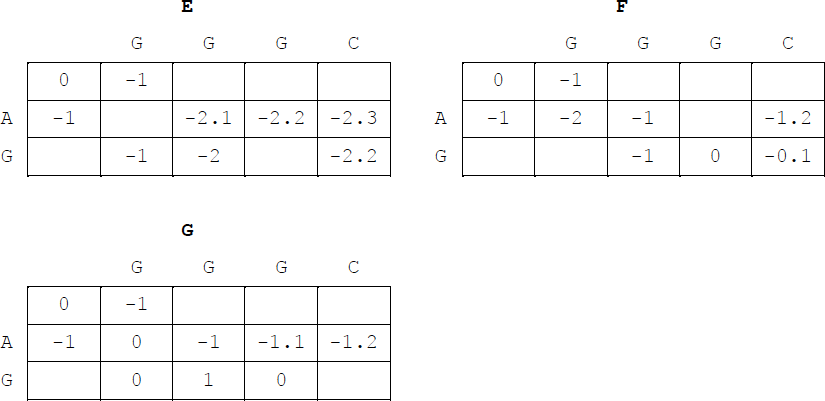
\includegraphics[width=0.75 \textwidth]{fig03/affine_dp_update.png}
\end{figure}

%% (b)
  \part
  What is the optimal score?

  \begin{solution}[0.35 in]
  $-0.1$
  \end{solution}
     
  \vspace{0.1 in}

\end{parts}

%%% Question 6
\question \textbf{Trackback with affine gap penalty}
  
Perform backtracking on E, F, and G tables to find the optimal alignment. The cells with double border should be visited during backtracking. 

\medskip 

\begin{figure}[h]
  \centering
      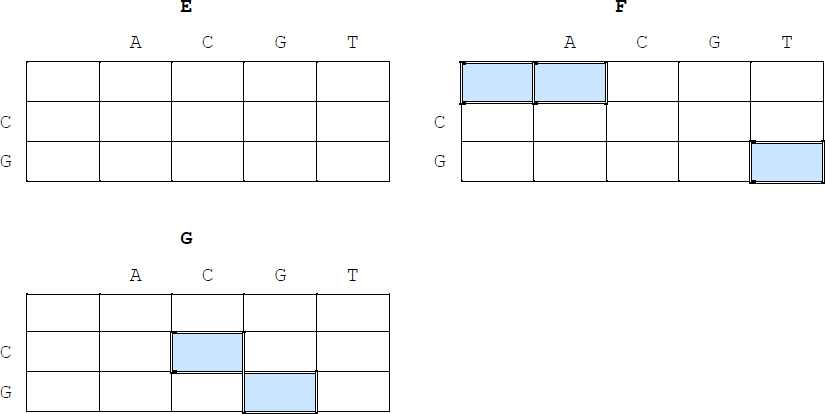
\includegraphics[width=0.75 \textwidth]{fig03/affine_dp_backtrack.png}
\end{figure}

\vspace{0.1 in}

\begin{parts}

%% (a)
  \part
   Write the optimal alignment.

  \begin{solution}[0.75 in]
  \begin{verbatim}
  q: -CG-
  d: ACGT
  \end{verbatim}
  \end{solution}

  \vspace{0.1 in}

\end{parts}

\newpage


%%% Question 7
\question \textbf{Sequence distance with DP}
DP can be used to calculate the edit distance (Levenshtein distance) between two sequences.

\medskip 

\textbf{Scoring scheme: }\\
\null \quad $R_{ab}$ = 0 for a = b \\ 
\null \quad $R_{ab}$ = -1 for a $\neq$ b \\ 
\null \quad $g = 1$

\vspace{0.1 in}


\vspace{0.1 in}

With the scoring scheme above, the edit distance d is calculated as $–1 * T$ where $T$ is the optimal score of the DP.

Find the edit distance between two sequences q = AG and d = ACG.

\begin{parts}

%% (a)
  \part
  Fill the DP table.
  
\begin{figure}[h]
  \centering
      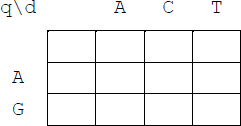
\includegraphics[width=0.35 \textwidth]{fig03/dp_distance.png}
\end{figure}

%% (b)
  \part
   What is the edit distance between q and d?

  \begin{solution}[0.35 in]
  \begin{verbatim}
  2
  \end{verbatim}
  \end{solution}

  \vspace{0.1 in}

\end{parts}


\end{questions}
%---------------------------------------------------------------------
       
\end{document}

